\question Find the path from the start, $S$, to the goal, $G$, when running
each of the following algorithms.

The \define{heuristic}, $h$, estimates the distance from each node to the goal.

\begin{center}
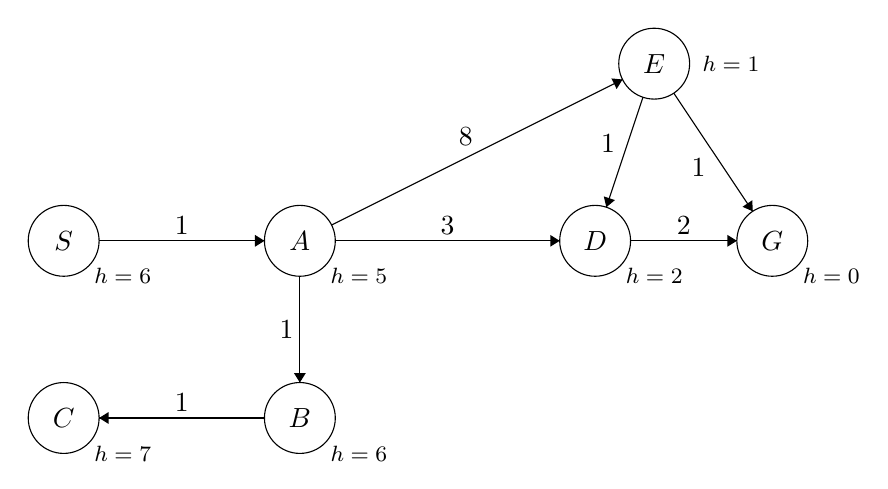
\begin{tikzpicture}[scale=0.15]
\tikzstyle{every node}+=[inner sep=0pt]
\draw (60,-15) circle (3);
\draw (60,-15) node {$E$};
\draw (66.5,-15) node {\footnotesize $h = 1$};
\draw (10,-30) circle (3);
\draw (10,-30) node {$S$};
\draw (15,-33) node {\footnotesize $h = 6$};
\draw (30,-30) circle (3);
\draw (30,-30) node {$A$};
\draw (35,-33) node {\footnotesize $h = 5$};
\draw (30,-45) circle (3);
\draw (30,-45) node {$B$};
\draw (35,-48) node {\footnotesize $h = 6$};
\draw (55,-30) circle (3);
\draw (55,-30) node {$D$};
\draw (60,-33) node {\footnotesize $h = 2$};
\draw (70,-30) circle (3);
\draw (70,-30) node {$G$};
\draw (75,-33) node {\footnotesize $h = 0$};
\draw (10,-45) circle (3);
\draw (10,-45) node {$C$};
\draw (15,-48) node {\footnotesize $h = 7$};
\draw (13,-30) -- (27,-30);
\fill (27,-30) -- (26.2,-29.5) -- (26.2,-30.5);
\draw (20,-29.5) node [above] {$1$};
\draw (30,-33) -- (30,-42);
\fill (30,-42) -- (30.5,-41.2) -- (29.5,-41.2);
\draw (29.5,-37.5) node [left] {$1$};
\draw (27,-45) -- (13,-45);
\fill (13,-45) -- (13.8,-45.5) -- (13.8,-44.5);
\draw (20,-44.5) node [above] {$1$};
\draw (33,-30) -- (52,-30);
\fill (52,-30) -- (51.2,-29.5) -- (51.2,-30.5);
\draw (42.5,-29.5) node [above] {$3$};
\draw (32.68,-28.66) -- (57.32,-16.34);
\fill (57.32,-16.34) -- (56.38,-16.25) -- (56.82,-17.15);
\draw (44.04,-22) node [above] {$8$};
\draw (59.05,-17.85) -- (55.95,-27.15);
\fill (55.95,-27.15) -- (56.68,-26.55) -- (55.73,-26.24);
\draw (56.73,-21.8) node [left] {$1$};
\draw (58,-30) -- (67,-30);
\fill (67,-30) -- (66.2,-29.5) -- (66.2,-30.5);
\draw (62.5,-29.5) node [above] {$2$};
\draw (61.66,-17.5) -- (68.34,-27.5);
\fill (68.34,-27.5) -- (68.31,-26.56) -- (67.48,-27.12);
\draw (64.39,-23.83) node [left] {$1$};
\end{tikzpicture}
\end{center}

\begin{parts}
\part Which path does Dijkstra's return?

\begin{solution}[1in]
$S - A - D - G$

From the starting node, choose the path that has the least cost, go to that
node, and repeat until we reach the goal node. We choose the lowest
\emph{total cost}.

We keep a priority-queue fringe that keeps track of paths. At each step, we
remove the shortest path from the fringe and add its children to the fringe,
trying all paths in increasing cost order until we reach $G$.
\end{solution}

\part Which path does A* search return?

\define{A* search} is an algorithm that combines the total distance from the
start with the heuristic to optimize the search procedure.

\begin{solution}[1in]
$S - A - D - G$

At each node, we choose the next node that has the lowest sum of the path cost
and $h(\cdot)$ value. This is essentially uniform cost search and greedy search
combined.

For A* to work, heuristics must be \emph{admissible} and \emph{consistent}.

\begin{itemize}
\item Admissible heuristics underestimate the true distance to the goal.
\item Consistent heuristics require that the difference in heuristic values
between two nodes cannot be greater than the true distance between the two.
\end{itemize}
\end{solution}

\part What is the runtime of Dijkstra's? A*? What is the space requirement for both?
\begin{solution}
  We assume a binary heap Priority Queue. The largest the PQ can ever get is size $V$ since there are $V$ vertices, and we never add vertices twice. (We update using \verb|decrementKey| instead.)

  In the worst case, we do the following in Dijkstra's:
  \begin{itemize}
    \item Insert every vertex into the PQ ($V$ vertexes, $O(\log{V})$ time)
    \item Remove every vertex from the PQ ($V$ vertexes, $O(\log{V})$ time)
    \item Update every vertex in the PQ ($E$ edges, $O(\log{V})$ time)
  \end{itemize}
  Hence, Dijkstra's has runtime $O(V\log{V} + V\log{V} + E\log{V}) = O(E\log{V})$ since $E > V$.

  A* has the same runtime as Dijkstra's in the worst case. We can see this by constructing a very poor heuristic that returns $0$ for all vertices! We can see that this heuristic is trivially admissible (distance to the goal is at least 0, so it must be admisible) and trivially consistent (the difference is always 0, which is not greater than the true distance between any two nodes). Then, the behaviour of A* on the graph is exactly like Dijkstra's.

  However, given a good heuristic, A* can have a better average runtime, which is why we often prefer it.

  The space requirement for the graph is $\Theta(V + E)$ assuming an adjacency list, and the space for the priority queue is $\Theta(V)$;
\end{solution}
\end{parts}
